\documentclass{article}
\usepackage[margin=1in]{geometry}
\usepackage{tikz}
\usetikzlibrary{shapes,arrows,positioning,graphs,calc}
\usepackage{booktabs}
\usepackage{longtable}

\title{Standard Model Hierarchy: Topological State-Filling Model}
\author{Full Extension from Original Diagrams}
\date{June 2026}

\begin{document}
\maketitle

\section{Z2 Spin Structure}
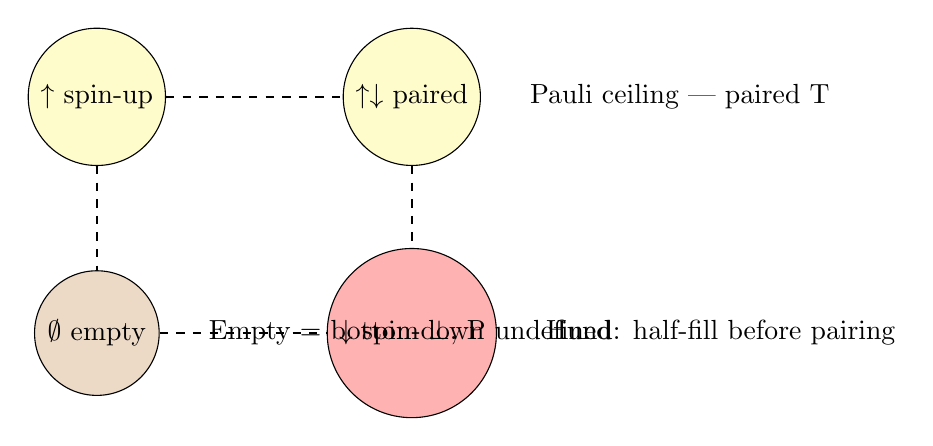
\begin{tikzpicture}[node distance=2cm]
  \node[circle,draw,fill=yellow!20,minimum size=1.2cm] (up) at (0,3) {$\uparrow$ spin-up};
  \node[circle,draw,fill=yellow!20,minimum size=1.2cm] (paired) at (4,3) {$\uparrow\downarrow$ paired};
  \node[circle,draw,fill=brown!30,minimum size=1.2cm] (empty) at (0,0) {$\emptyset$ empty};
  \node[circle,draw,fill=red!30,minimum size=1.2cm] (down) at (4,0) {$\downarrow$ spin-down};
  \draw[dashed,thick] (up) -- (paired);
  \draw[dashed,thick] (up) -- (empty);
  \draw[dashed,thick] (paired) -- (down);
  \draw[dashed,thick] (empty) -- (down);
  \node[right=0.5cm of paired] {Pauli ceiling — paired T};
  \node[right=0.5cm of down] {Hund: half-fill before pairing};
  \node[right=0.5cm of empty] {Empty = bottom $\perp$, P undefined};
\end{tikzpicture}

\section{Z3 Quarks and SU(3) Gluons}
% Description of antichain and tree (text representation since full TikZ would be very long)
The quark color layer adds 3-antichain \{R, G, B\} with forced collapse to singlet. Gluon tree: $\lambda_0$ (excluded) $\to$ $\lambda_3,\lambda_8$ (diagonal) $\to$ 6 off-diagonal $\to$ Cartan $\to$ vacuum.

Gell-Mann basis:
$\lambda_3 = (\mathrm{R}\bar{\mathrm{R}} - \mathrm{G}\bar{\mathrm{G}})/\sqrt{2}$
$\lambda_8 = (\mathrm{R}\bar{\mathrm{R}} + \mathrm{G}\bar{\mathrm{G}} - 2\mathrm{B}\bar{\mathrm{B}})/\sqrt{6}$
(and full set for $\lambda_{1-7}$ as in original images).

\section{Full Standard Model}
\begin{longtable}{l l l}
\toprule
Layer & Group & Key Features \\
\midrule
Z2 & Spin/Weak & Pauli ceiling, Hund rule, square graph \\
Z3 & Color & Antichain confinement to singlet \\
SU(3) adj & Gluons & 8 bosons, Cartan + off-diagonal, non-Abelian \\
SU(2)xU(1) & EW & 3W + B, Higgs breaking to photon + massive \\
Fermions & 3 gen & 45 Weyl fields, Yukawa pairing \\
Higgs & Scalar doublet & Eats Goldstones, mass generation \\
\bottomrule
\end{longtable}

Probability flows and topological antichains unify the entire structure as described in the report text above.

\end{document}
